% $Id: testing.tex 6081 2018-06-15 21:04:52Z mskala $

%
% MSK 012 testing and instructions
% Copyright (C) 2018  Matthew Skala
%
% This program is free software: you can redistribute it and/or modify
% it under the terms of the GNU General Public License as published by
% the Free Software Foundation, version 3.
%
% This program is distributed in the hope that it will be useful,
% but WITHOUT ANY WARRANTY; without even the implied warranty of
% MERCHANTABILITY or FITNESS FOR A PARTICULAR PURPOSE.  See the
% GNU General Public License for more details.
%
% You should have received a copy of the GNU General Public License
% along with this program.  If not, see <http://www.gnu.org/licenses/>.
%
% Matthew Skala
% https://northcoastsynthesis.com/
% mskala@northcoastsynthesis.com
%
\chapter{Testing}

The MSK~012 needs no trimming or adjustment; unless there are defective
components or build errors, it should work as soon as it's built.  But here
are some notes on testing and troubleshooting.

\section{Short-circuit test}

With no power applied to the module, check for short circuits between the
three power connections on the Eurorack power connector.  The two pins at
the bottom, marked with white on the circuit board, are for -12V.  The two
at the other end are for +12V; and the remaining six pins in the middle are
all ground pins.  Check between each pairing of these three voltages, in
both directions (six tests in all).  Ideally, you should use a multimeter's
``diode test'' range for this; if yours has no such range, use a low
resistance-measuring setting.  It should definitely read infinite in the
reverse direction (positive lead to $-$12V and negative lead to each of the
other two, as well as positive lead to ground and negative to $+$12V) and it
will probably read infinite, but at least
greater than 1V or 1k$\Omega$, in the forward direction (reverse those three
tests).  If any of these six measurements is less than 1k$\Omega$ or 1V,
then something is wrong with the build, most likely a blob of solder
shorting between two connections, and you should troubleshoot that before
applying power.

\emph{Optional}:  Although we test all cables before we sell them, bad
cables have been known to exist, so it might be worth plugging the Eurorack
power cable into the module and repeating these continuity tests across the
cable's corresponding contacts (using bits of narrow-gauge wire to get into
the contacts on the cable if necessary, or probing the pins of the power
connector on the back side of the circuit board) to make sure there are no
shorts in the cable crimping.  Doing this test \emph{with the cable
connected to the module} makes it easier to avoid mistakes, because the
module itself will short together all wires that carry equal potential,
making it easier to be sure of testing the relevant adjacent-wire pairs in
the cable.

Plug the module into a Eurorack power supply and make sure
neither it nor the power supply emits smoke, overheats, makes any unusual
noises, or smells bad.  If any of those things happen, turn off the power
immediately, and troubleshoot the problem before proceeding.

\emph{Optional}: Plug the module into a Eurorack power supply
\emph{backwards}, see that nothing bad happens, and congratulate yourself on
having assembled the reverse-connection protective circuit properly. 
Reconnect it right way round before proceeding to the next step.

\section{Envelope shape}

If you have access to an oscilloscope and pulse-wave LFO:  apply power to
the module, feed a pulse wave of about 10Hz into the input, set the range
switch to the middle (fastest) position, and look at the output with the
oscilloscope.  It should look like some sort of reasonable ADSR envelope,
and it should change as expected when you adjust the knobs.

\noindent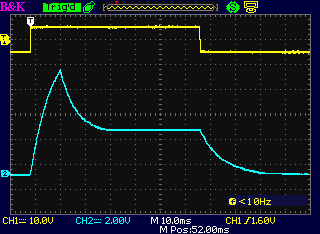
\includegraphics[width=\linewidth]{BK000032.png}

It is possible, and normal, for the ``zero'' voltage between pulses to
appear a fraction of a volt less than zero, especially when there is no load
on the output except a high-impedance scope probe.  It is also possible that
the maximum sustain level (S knob turned fully clockwise) may be a little
higher than the attack peak, resulting in an unusual-looking envelope shape.

\section{Troubleshooting}

Some common problems to look for if something goes wrong:
\begin{itemize}
  \item Solder bridges, especially between closely-spaced joints on TO-92
    transistors.
  \item Other solder problems, such as solder not sticking to the board (can
    be caused by too-high iron temperatures, or the wrong flux).
  \item Polarized components installed backwards.
  \item Components swapped around, such as the
    100k$\Omega$ panel pot installed in the wrong one of the four spots (the
    other three requiring similar-looking 1M$\Omega$ pots), or swapping the
    27k$\Omega$ resistor with one of its 270k$\Omega$ cousins.
  \item User error (misunderstanding the intended operation of the module),
    such as missing the sustain phase when the sustain level is set fully
    counterclockwise, or using short triggers on the input with slow
    envelope settings.
\end{itemize}

During development an issue was noted between this module and the Befaco
Rampage.  The Rampage's gate output apparently never went quite to zero
volts, remaining at a high enough positive voltage in between gates that the
MSK~012 never recognized the end of the gate.  The final released design of
the MSK~012 has had its gate thresholds raised to help prevent such issues,
and that seemed to fix the problem; but in general, do be aware that it
cannot work miracles in the case of faulty input, and the transistor Schmitt
trigger at the input does require some nonzero amount of current-sinking
(not just an open circuit) in the low state.  The Rampage's outputs have
been known to cause problems with other modules before, because in the low
state they connect to ground only through an LED, presenting a high
impedance at voltages below about one
volt.\footnote{\url{https://www.muffwiggler.com/forum/viewtopic.php?t=187044}}
